\documentclass{article}
\usepackage[utf8]{inputenc}
\usepackage[spanish]{babel}
\usepackage{graphicx}
\usepackage{longtable}
\usepackage{float}
\usepackage{amsmath}
\graphicspath{{./img/}}

\title{Práctica 2. Algoritmos divide y vencerás - Suma de dos elementos}

\author{Noelia Escalera Mejías \\
		\and Alejandro Menor Molinero \\
		\and Javier Núñez Suárez \\
		\and Adra Sánchez Ruiz \\
		\and Jesús Torres Sánchez}
\begin{document}
	\maketitle
	\section{Introducción}
	El problema que se nos plantea en esta práctica es, a grandes rasgos, el de encontrar dos elementos en un vector que sumen un valor específico.
	
	
	\subsection{Eficiencia teórica: algoritmo básico}
	
	El algoritmo obvio, utiliza dos bucles anidados para probar todas las posibilidades del vector hasta encontrar una pareja que sume el valor dado como parámetro.
	Este algoritmo es de orden cuadrático $O(n^2)$.
	
	
	\subsection{Eficiencia teórica: algoritmo DyV}
	Para aplicar la técnica divide y vencerás necesitamos tener alguna certeza sobre los elementos del vector y así dividir el problema en subproblemas. Como estos son generados aleatoriamente, necesitamos ordenarlos.
	Para esto, hacemos uso del algoritmo Quicksort.
	
	\
	Una vez ordenado el vector, el algoritmo Divide y Vencerás realiza la suma del primer elemento y el último del vector.
	
	\
	
	A partir de ahi pueden ocurrir tres cosas:
	\begin{itemize}
		\item Que la suma sea el valor que estamos buscando.
		\item Que la suma sea menor que el valor que estamos buscando.
		\item Que la suma sea mayor que el valor que estamos buscando.
	\end{itemize}

	Si se da el primer caso devolvemos esta solución, de lo contrario, realizamos una llamada recursiva con los mismos elementos menos el primero o el último elemento respectivamente.
	\
	
	Hemos calculado la eficiencia teórica de esta parte del algoritmo, mediante el método de expansión. Este método  consiste en desarrollar progresivamente la ecuación de recurrencia para diversos niveles sustituyendo cada aparición del valor de la función por la expresión que se especifica en la recurrencia. Es necesario identificar un patrón general, y aplicarlo para resolver.
	

\begin{align*}
	T(n) &= T(n-1) + c \\
	T(n) &= T(n-2) + 2c \\
	T(n) &= T(n-i) + ic \\
		(i &= n - 2) \\
	T(n) &= T(2) + (n-2)c \\
	T(n) &= cn + k - 2c
\end{align*}
Como acabamos de demostrar el orden de eficiencia de esta parte es $O(n)$.
	Como resultado, el orden de eficiencia total es el máximo de los dos segmentos en los que hemos dividido el problema. Como Quicksort está acotado por $O(n*log n)$ y el de
nuestro algoritmo por $O(n)$, \textbf{la eficiencia conjunta es de orden $O(n*log n)$} ya que este es 
dominante.
	\section{Análisis de eficiencia empírica}
	Vamos a medir el tiempo que tardan en ejecutarse los dos algoritmos:
	
	\
	Además, los compararemos entre ellos cuando sea interesante hacerlo.
	
	\
	He aquí una tabla comparativa del tiempo que tarda cada algoritmo según el tamaño del vector a ordenar.
	
	\begin{longtable}{|c|c|c|}
		\hline
		Tamaño del vector & Tiempos con algoritmo obvio & Tiempos con algoritmo divide y vencerás \\ \hline
		2	    &  1.2924e-07 	 &  2,63E-04  \\ \hline
		52	    &  1.07248e-05	 &  1.26865e-05  \\ \hline                  
		102	    &  3.50414e-05	 &  2.67046e-05  \\ \hline                  
		152	    &  7.59376e-05	 &  4.1936e-05   \\ \hline                 
		202	    &  5.56089e-05	 &  5.73871e-05  \\ \hline                  
		252	    &  7.89973e-05	 &  2.08299e-05  \\ \hline                  
		302	    &  0.00010781 	 &  2.17031e-05  \\ \hline                  
		352	    &  0.000140278	 &  2.98889e-05  \\ \hline                  
		402	    &  0.000182669	 &  3.08486e-05  \\ \hline                  
		452	    &  0.000229592	 &  3.52622e-05  \\ \hline                  
		502	    &  0.000282326	 &  3.94338e-05  \\ \hline                  
		552	    &  0.000340752	 &  4.5054e-05   \\ \hline                 
		602	    &  0.000404462	 &  4.84906e-05  \\ \hline                  
		652	    &  0.000474133	 &  5.30354e-05  \\ \hline                  
		702	    &  0.000550061	 &  5.8354e-05   \\ \hline                 
		752	    &  0.000633286	 &  6.2162e-05   \\ \hline                 
		802	    &  0.000752916	 &  6.72947e-05  \\ \hline                  
		852	    &  0.000806551	 &  7.07294e-05  \\ \hline                  
		902	    &  0.000903983	 &  7.62306e-05  \\ \hline                  
		952	    &  0.00101016 	 &  8.07653e-05  \\ \hline                  
		1002	&  0.00112748 	 &  8.53134e-05  \\ \hline                  
		1052	&  0.00122338 	 &  8.82979e-05  \\ \hline                  
		1102	&  0.00133783 	 &  9.37333e-05  \\ \hline                  
		1152	&  0.00147163 	 &  9.93348e-05  \\ \hline                  
		1202	&  0.00161119 	 &  0.000102006  \\ \hline                  
		1252	&  0.00172966 	 &  0.000107358  \\ \hline                  
		1302	&  0.00187488 	 &  0.000113005  \\ \hline                  
		1352	&  0.0020381  	 &  0.000116932  \\ \hline                  
		1402	&  0.00216357 	 &  0.000120731  \\ \hline                  
		1452	&  0.0023202  	 &  0.000128124  \\ \hline                  
		1502	&  0.00254558 	 &  0.000131672  \\ \hline                  
		1552	&  0.00265279 	 &  0.000136404  \\ \hline                  
		1602	&  0.00283962 	 &  0.000140153  \\ \hline                  
		1652	&  0.0030034  	 &  0.000145704  \\ \hline                  
		1702	&  0.00322624 	 &  0.000151027  \\ \hline                  
		1752	&  0.00337908 	 &  0.000156419  \\ \hline                  
		1802	&  0.00359821 	 &  0.000162374  \\ \hline                  
		1852	&  0.00378694 	 &  0.000168315  \\ \hline                  
		1902	&  0.00401242 	 &  0.000171145  \\ \hline                  
		1952	&  0.00421789 	 &  0.00017807   \\ \hline                 
		2002	&  0.00443473 	 &  0.000181655  \\ \hline                  
		2052	&  0.00466831 	 &  0.000190365  \\ \hline                  
		2102	&  0.00485557 	 &  0.000193026  \\ \hline                  
		2152	&  0.00511763 	 &  0.000197088  \\ \hline                  
		2202	&  0.00543528 	 &  0.000199874  \\ \hline                  
		2252	&  0.00560486 	 &  0.00021286   \\ \hline                 
		2302	&  0.00585189 	 &  0.000212914  \\ \hline                  
		2352	&  0.00611448 	 &  0.000218924  \\ \hline                  
		2402	&  0.00636008 	 &  0.000221981  \\ \hline                  
		2452	&  0.00660472 	 &  0.00022756   \\ \hline                 
		2502	&  0.00698231 	 &  0.000231273  \\ \hline                  
		2552	&  0.00715784 	 &  0.000236687  \\ \hline                  
		2602	&  0.00746965 	 &  0.000254065  \\ \hline                  
		2652	&  0.00774443 	 &  0.000254985  \\ \hline                  
		2702	&  0.00805125 	 &  0.00025201   \\ \hline                 
		2752	&  0.00834981 	 &  0.000256611  \\ \hline                  
		2802	&  0.00866045 	 &  0.000263844  \\ \hline                  
		2852	&  0.00895092 	 &  0.000275502  \\ \hline                  
		2902	&  0.00927373 	 &  0.000275377  \\ \hline                  
		2952	&  0.00961669 	 &  0.000277578  \\ \hline                  
		3002	&  0.0100844  	 &  0.000288198  \\ \hline                  
		3052	&  0.0102326  	 &  0.000293423  \\ \hline                  
		3102	&  0.0106085  	 &  0.000294533  \\ \hline                  
		3152	&  0.0110291  	 &  0.000300316  \\ \hline                  
		3202	&  0.0112732  	 &  0.000304138  \\ \hline                  
		3252	&  0.0117902  	 &  0.000310318  \\ \hline                  
		3302	&  0.0120512  	 &  0.000327855  \\ \hline                  
		3352	&  0.0124521  	 &  0.000331585  \\ \hline                  
		3402	&  0.0127606  	 &  0.000327506  \\ \hline                  
		3452	&  0.0131763  	 &  0.000335943  \\ \hline                  
		3502	&  0.0137258  	 &  0.000342597  \\ \hline                  
		3552	&  0.014027   	 &  0.00035208   \\ \hline                 
		3602	&  0.0142926  	 &  0.000363522  \\ \hline                  
		3652	&  0.0146585  	 &  0.000372     \\ \hline               
		3702	&  0.0150581  	 &  0.000388923  \\ \hline                  
		3752	&  0.0154795  	 &  0.000383769  \\ \hline                  
		3802	&  0.015958   	 &  0.000388151  \\ \hline                  
		3852	&  0.0163076  	 &  0.000392653  \\ \hline                  
		3902	&  0.0167318  	 &  0.000394175  \\ \hline                  
		3952	&  0.0176898  	 &  0.000402757  \\ \hline                  
		4002	&  0.0188954  	 &  0.000410174  \\ \hline                  
		4052	&  0.0187919  	 &  0.00040309   \\ \hline                 
		4102	&  0.0192961  	 &  0.000405281  \\ \hline                  
		4152	&  0.0196487  	 &  0.000423668  \\ \hline                  
		4202	&  0.0208504  	 &  0.000415645  \\ \hline                  
		4252	&  0.0212144  	 &  0.000420764  \\ \hline                  
		4302	&  0.0223817  	 &  0.000427357  \\ \hline                  
		4352	&  0.0219622  	 &  0.000432821  \\ \hline                  
		4402	&  0.0226035  	 &  0.000438693  \\ \hline                  
		4452	&  0.0225804  	 &  0.000458516  \\ \hline                  
		4502	&  0.0234626  	 &  0.000464868  \\ \hline                  
		4552	&  0.0245493  	 &  0.000498882  \\ \hline                  
		4602	&  0.0244892  	 &  0.000508813  \\ \hline                  
		4652	&  0.0253656  	 &  0.000499163  \\ \hline                  
		4702	&  0.0253671  	 &  0.000488681  \\ \hline                  
		4752	&  0.0249446  	 &  0.000496277  \\ \hline                  
		4802	&  0.0252559  	 &  0.000499227  \\ \hline                  
		4852	&  0.0258745  	 &  0.000507609  \\ \hline                  
		4902	&  0.0267505  	 &  0.000508594  \\ \hline                  
		4952	&  0.0279315  	 &  0.000530366  \\ \hline                  
		5002	&  0.0285257  	 &  0.000553612  \\ \hline                  
		5052	&  0.0289256  	 &  0.00053935   \\ \hline                 
		5102	&  0.0286501  	 &  0.000557164  \\ \hline                  
		5152	&  0.029081   	 &  0.000551248  \\ \hline                  
		5202	&  0.0298208  	 &  0.000547572  \\ \hline                  
		5252	&  0.0303569  	 &  0.00055586   \\ \hline                 
		5302	&  0.0308366  	 &  0.000543844  \\ \hline                  
		5352	&  0.0314377  	 &  0.000568829  \\ \hline                  
		5402	&  0.032035   	 &  0.000580758  \\ \hline                  
		5452	&  0.0326124  	 &  0.000582503  \\ \hline                  
		5502	&  0.0335289  	 &  0.000591532  \\ \hline                  
		5552	&  0.0337874  	 &  0.000562229  \\ \hline                  
		5602	&  0.0345751  	 &  0.000569521  \\ \hline                  
		5652	&  0.035593   	 &  0.000576387  \\ \hline                  
		5702	&  0.0359639  	 &  0.000585342  \\ \hline                  
		5752	&  0.0362786  	 &  0.000604199  \\ \hline                  
		5802	&  0.0369571  	 &  0.000630955  \\ \hline                  
		5852	&  0.0401922  	 &  0.000632735  \\ \hline                  
		5902	&  0.0413387  	 &  0.000620298  \\ \hline                  
		5952	&  0.0404016  	 &  0.000622768  \\ \hline                  
		6002	&  0.0427071  	 &  0.00064486   \\ \hline                 
		6052	&  0.0418601  	 &  0.000644819  \\ \hline                  
		6102	&  0.0412707  	 &  0.000661322  \\ \hline                  
		6152	&  0.041784   	 &  0.000626894  \\ \hline                  
		6202	&  0.043056   	 &  0.000634944  \\ \hline                  
		6252	&  0.043146   	 &  0.000641708  \\ \hline                  
		6302	&  0.0460017  	 &  0.000646953  \\ \hline                  
		6352	&  0.0458783  	 &  0.000658047  \\ \hline                  
		6402	&  0.0471116  	 &  0.0006529    \\ \hline                
		6452	&  0.0489031  	 &  0.000726562  \\ \hline                  
		6502	&  0.0480484  	 &  0.000711373  \\ \hline                  
		6552	&  0.0506584  	 &  0.000825281  \\ \hline                  
		6602	&  0.0490175  	 &  0.000868788  \\ \hline                  
		6652	&  0.0498296  	 &  0.000754546  \\ \hline                  
		6702	&  0.0525766  	 &  0.000717796  \\ \hline                  
		6752	&  0.0517779  	 &  0.000710808  \\ \hline                  
		6802	&  0.0531025  	 &  0.000708588  \\ \hline                  
		6852	&  0.0526342  	 &  0.000712429  \\ \hline                  
		6902	&  0.0554639  	 &  0.000723362  \\ \hline                  
		6952	&  0.0535908  	 &  0.000719322  \\ \hline                  
		7002	&  0.0565233  	 &  0.000768295  \\ \hline                  
		7052	&  0.0574797  	 &  0.000782286  \\ \hline                  
		7102	&  0.0579865  	 &  0.000793095  \\ \hline                  
		7152	&  0.0593768  	 &  0.000792248  \\ \hline                  
		7202	&  0.0576529  	 &  0.000808728  \\ \hline                  
		7252	&  0.0592291  	 &  0.000811163  \\ \hline                  
		7302	&  0.0604172  	 &  0.000822073  \\ \hline                  
		7352	&  0.0603504  	 &  0.000813531  \\ \hline                  
		7402	&  0.0604276  	 &  0.0008125    \\ \hline                
		7452	&  0.0619357  	 &  0.000868281  \\ \hline                  
		7502	&  0.0653653  	 &  0.000849655  \\ \hline                  
		7552	&  0.0664603  	 &  0.000827294  \\ \hline                  
		7602	&  0.0680857  	 &  0.000815002  \\ \hline                  
		7652	&  0.0671396  	 &  0.00080591   \\ \hline                 
		7702	&  0.0683615  	 &  0.000811489  \\ \hline                  
		7752	&  0.0695572  	 &  0.000844817  \\ \hline                  
		7802	&  0.069214   	 &  0.000860518  \\ \hline                  
		7852	&  0.0699345  	 &  0.000858407  \\ \hline                  
		7902	&  0.0714936  	 &  0.000858995  \\ \hline                  
		7952	&  0.0715503  	 &  0.000846543  \\ \hline                  
		8002	&  0.0739281  	 &  0.000842728  \\ \hline                  
		8052	&  0.0749469  	 &  0.000859317  \\ \hline                  
		8102	&  0.0749397  	 &  0.000853653  \\ \hline                  
		8152	&  0.078582   	 &  0.000859815  \\ \hline                  
		8202	&  0.0782962  	 &  0.000871943  \\ \hline                  
		8252	&  0.078807   	 &  0.000885368  \\ \hline                  
		8302	&  0.0801562  	 &  0.000892515  \\ \hline                  
		8352	&  0.0798039  	 &  0.000887462  \\ \hline                  
		8402	&  0.0797402  	 &  0.000891047  \\ \hline                  
		8452	&  0.0816974  	 &  0.0008969    \\ \hline                
		8502	&  0.0823709  	 &  0.000901171  \\ \hline                  
		8552	&  0.081603   	 &  0.000910187  \\ \hline                  
		8602	&  0.0810998  	 &  0.000915118  \\ \hline                  
		8652	&  0.0827913  	 &  0.000914494  \\ \hline                  
		8702	&  0.0854845  	 &  0.000919405  \\ \hline                  
		8752	&  0.0875262  	 &  0.000930408  \\ \hline                  
		8802	&  0.0875256  	 &  0.000933171  \\ \hline                  
		8852	&  0.0876953  	 &  0.000943334  \\ \hline                  
		8902	&  0.0877304  	 &  0.000954054  \\ \hline                  
		8952	&  0.0878086  	 &  0.000988322  \\ \hline                  
		9002	&  0.0890702  	 &  0.00100255   \\ \hline                 
		9052	&  0.0914813  	 &  0.00101775   \\ \hline                 
		9102	&  0.0917751  	 &  0.00101937   \\ \hline                 
		9152	&  0.0913303  	 &  0.0010266    \\ \hline                
		9202	&  0.0926901  	 &  0.0010076    \\ \hline                
		9252	&  0.0991961  	 &  0.0010183    \\ \hline                
		9302	&  0.103345   	 &  0.0010104    \\ \hline                
		9352	&  0.101013   	 &  0.00104976   \\ \hline                 
		9402	&  0.101412   	 &  0.00104057   \\ \hline                 
		9452	&  0.0982718  	 &  0.00104326   \\ \hline                 
		9502	&  0.0994359  	 &  0.00102554   \\ \hline                 
		9552	&  0.100967   	 &  0.00102609   \\ \hline                 
		9602	&  0.103773   	 &  0.00103448   \\ \hline                 
		9652	&  0.105992   	 &  0.001034     \\ \hline               
		9702	&  0.105317   	 &  0.0010377    \\ \hline                
		9752	&  0.105496   	 &  0.00105498   \\ \hline                 
		9802	&  0.107417   	 &  0.00105341   \\ \hline                 
		9852	&  0.110844   	 &  0.00106947   \\ \hline                 
		9902	&  0.113998   	 &  0.00106406   \\ \hline                 
		9952	&  0.112215   	 &  0.00106635   \\ \hline     
	\end{longtable}
	
	\section{Análisis de eficiencia híbrida}
	Ajuste de los algoritmos de acuerdo a su eficiencia teórica y los datos obtenidos en la eficiencia empírica.
	
	\subsection{Ajuste del algoritmo básico}
	
	\begin{longtable}{|c|c|c|}
		\hline
		Constante		& Valor			& Error estándar	\\ \hline
		a0              & 1.12169e-09	& 0.9625 \\ \hline
		a1              & 1.10848e-07	& 100.2	 \\ \hline
		a2              & -0.000225747	& 106	 \\ \hline
	\end{longtable}
	
	\begin{figure}[H]
		\centering
		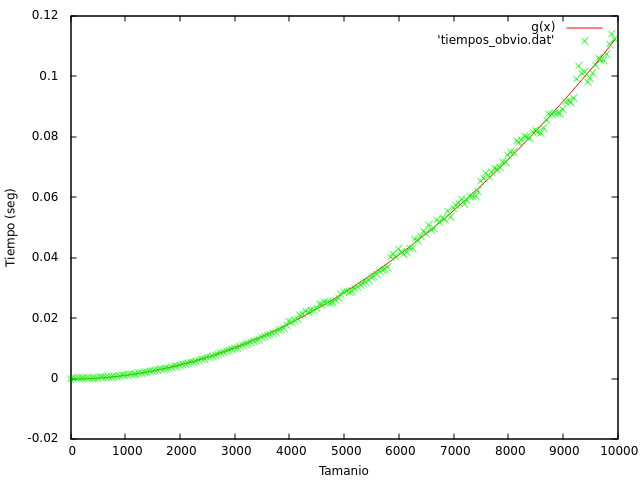
\includegraphics[totalheight=8cm]{img/Basico_ajustada}
		\caption{Ajuste algoritmo básico}
		\label{fig:Basico_ajustada}
	\end{figure}
	
	\subsection{Ajuste del algoritmo Divide y Vencerás}
	
	\begin{longtable}{|c|c|c|}
		\hline
		Constante		& Valor			& Error estándar	\\ \hline
		b0              & 7.472e-09		& 22.27	 \\ \hline
		b1              & 4.17793e-08 	& 37.34	 \\ \hline
		b2              & -6.70324e-06	& 94.89	 \\ \hline
	\end{longtable}
	
	\begin{figure}[H]
		\centering
		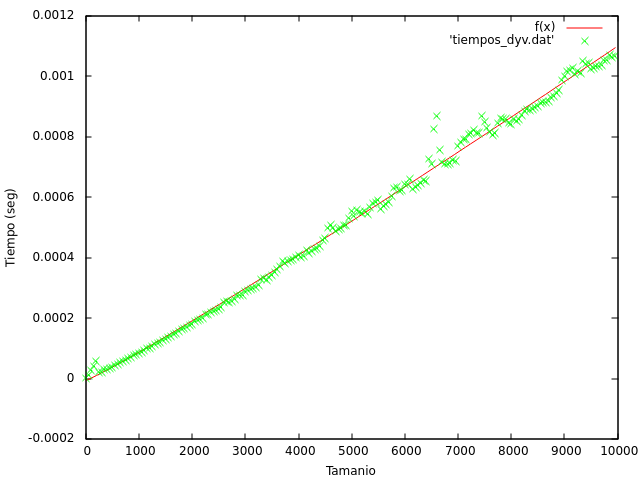
\includegraphics[totalheight=8cm]{img/DyV_ajustada}
		\caption{Ajuste algoritmo Divide y Vencerás}
		\label{fig:DyV_ajustada}
	\end{figure}
	
	Comparativas entre funciones:
	
	\begin{figure}[H]
		\centering
		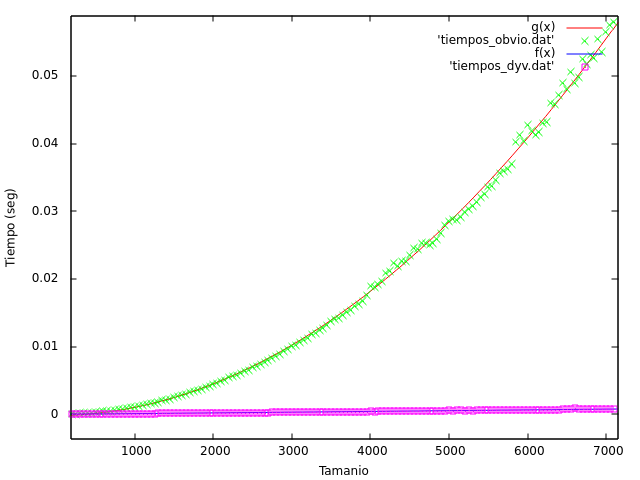
\includegraphics[totalheight=8cm]{img/ajustes_total}
		\caption{Ajustes comparativos}
		\label{fig:ajustes_total}
	\end{figure}
	\section{El precio de la recurrencia}

	\begin{longtable}{|c|c|c|c|}
		\hline
		Tamaño del vector & Tiempo con el alg. recursivo & Tiempo con el alg. iterativo & Cociente entre tiempos \\ \hline 
		2	    &   2.63E-04	  & 2.23E-04	 &  1.17937219730942   \\ \hline
		52	    &   1.27E-05	  & 6.13E-06	 &  2.06936318127175   \\ \hline
		102	    &   2.67E-05	  & 1.29E-05	 &  2.06858461919812   \\ \hline
		152	    &   4.19E-05	  & 2.03E-05	 &  2.06970752845256   \\ \hline
		202	    &   5.74E-05	  & 2.82E-05	 &  2.03770603566432   \\ \hline
		252	    &   2.08E-05	  & 3.90E-05	 &  0.533876866847958   \\ \hline
		302	    &   2.17E-05	  & 2.83E-05	 &  0.768177908660057   \\ \hline
		352	    &   2.99E-05	  & 2.52E-05	 &  1.18816560990638   \\ \hline
		402	    &   3.08E-05	  & 3.35E-05	 &  0.92060915159853   \\ \hline
		452	    &   3.53E-05	  & 3.53E-05	 &  0.999897918096286   \\ \hline
		502	    &   3.94E-05	  & 3.95E-05	 &  0.997510889856876   \\ \hline
		552	    &   4.51E-05	  & 4.18E-05	 &  1.07860036197535   \\ \hline
		602	    &   4.85E-05	  & 4.67E-05	 &  1.03861394197199   \\ \hline
		652	    &   5.30E-05	  & 5.04E-05	 &  1.0524254120075   \\ \hline
		702	    &   5.84E-05	  & 5.47E-05	 &  1.06599392781332   \\ \hline
		752	    &   6.22E-05	  & 5.93E-05	 &  1.04891045738179   \\ \hline
		802	    &   6.73E-05	  & 6.38E-05	 &  1.05546571975727   \\ \hline
		852	    &   7.07E-05	  & 6.77E-05	 &  1.04423532329788   \\ \hline
		902	    &   7.62E-05	  & 7.61E-05	 &  1.00227459188825   \\ \hline
		952	    &   8.08E-05	  & 7.89E-05	 &  1.02306948841015   \\ \hline
		1002	&   8.53E-05	  & 8.35E-05	 &  1.02213846183338   \\ \hline
		1052	&   8.83E-05	  & 8.88E-05	 &  0.994514833040303   \\ \hline
		1102	&   9.37E-05	  & 9.28E-05	 &  1.00986884988036   \\ \hline
		1152	&   9.93E-05	  & 9.70E-05	 &  1.02359418455955   \\ \hline
		1202	&   0.000102006	  & 1.00E-04	 &  1.02009978389157   \\ \hline
		1252	&   0.000107358	  & 0.000103916	 &  1.03312290696332   \\ \hline
		1302	&   0.000113005	  & 0.00010925	 &  1.03437070938215   \\ \hline
		1352	&   0.000116932	  & 0.000113826	 &  1.02728726301548   \\ \hline
		1402	&   0.000120731	  & 0.000118393	 &  1.01974778914294   \\ \hline
		1452	&   0.000128124	  & 0.000122945	 &  1.04212452722762   \\ \hline
		1502	&   0.000131672	  & 0.000127366	 &  1.03380808064947   \\ \hline
		1552	&   0.000136404	  & 0.00013242	 &  1.03008608971454   \\ \hline
		1602	&   0.000140153	  & 0.000136411	 &  1.02743180535294   \\ \hline
		1652	&   0.000145704	  & 0.000142313	 &  1.0238277599376   \\ \hline
		1702	&   0.000151027	  & 0.000146299	 &  1.03231737742568   \\ \hline
		1752	&   0.000156419	  & 0.000150775	 &  1.03743326148234   \\ \hline
		1802	&   0.000162374	  & 0.000161107	 &  1.00786433860726   \\ \hline
		1852	&   0.000168315	  & 0.000170044	 &  0.989832043471102   \\ \hline
		1902	&   0.000171145	  & 0.000170165	 &  1.00575911615197   \\ \hline
		1952	&   0.00017807	  & 0.000186775	 &  0.953393120064249   \\ \hline
		2002	&   0.000181655	  & 0.000183533	 &  0.98976750775065   \\ \hline
		2052	&   0.000190365	  & 0.00018714	 &  1.01723308752805   \\ \hline
		2102	&   0.000193026	  & 0.000194033	 &  0.994810161158153   \\ \hline
		2152	&   0.000197088	  & 0.000199301	 &  0.98889619219171   \\ \hline
		2202	&   0.000199874	  & 0.00020092	 &  0.994793947839936   \\ \hline
		2252	&   0.00021286	  & 0.00020046	 &  1.06185772722738   \\ \hline
		2302	&   0.000212914	  & 0.000204847	 &  1.03938061089496   \\ \hline
		2352	&   0.000218924	  & 0.000210554	 &  1.03975227257616   \\ \hline
		2402	&   0.000221981	  & 0.000215934	 &  1.02800392712588   \\ \hline
		2452	&   0.00022756	  & 0.000220837	 &  1.03044326811177   \\ \hline
		2502	&   0.000231273	  & 0.000224179	 &  1.03164435562653   \\ \hline
		2552	&   0.000236687	  & 0.000229298	 &  1.0322244415564   \\ \hline
		2602	&   0.000254065	  & 0.000236982	 &  1.07208564363538   \\ \hline
		2652	&   0.000254985	  & 0.000254445	 &  1.00212226610859   \\ \hline
		2702	&   0.00025201	  & 0.000252719	 &  0.997194512482243   \\ \hline
		2752	&   0.000256611	  & 0.000258336	 &  0.99332264957265   \\ \hline
		2802	&   0.000263844	  & 0.000262392	 &  1.00553370529589   \\ \hline
		2852	&   0.000275502	  & 0.000262609	 &  1.04909580402804   \\ \hline
		2902	&   0.000275377	  & 0.000266272	 &  1.03419435764932   \\ \hline
		2952	&   0.000277578	  & 0.000284482	 &  0.975731329222938   \\ \hline
		3002	&   0.000288198	  & 0.000280591	 &  1.02711063433966   \\ \hline
		3052	&   0.000293423	  & 0.000279477	 &  1.04990034958154   \\ \hline
		3102	&   0.000294533	  & 0.000285245	 &  1.03256148223457   \\ \hline
		3152	&   0.000300316	  & 0.000291832	 &  1.02907152060089   \\ \hline
		3202	&   0.000304138	  & 0.000294516	 &  1.03267055100572   \\ \hline
		3252	&   0.000310318	  & 0.000301658	 &  1.02870800708087   \\ \hline
		3302	&   0.000327855	  & 0.000305699	 &  1.07247652102231   \\ \hline
		3352	&   0.000331585	  & 0.000310644	 &  1.0674115708013   \\ \hline
		3402	&   0.000327506	  & 0.000328134	 &  0.998086147732329   \\ \hline
		3452	&   0.000335943	  & 0.000330577	 &  1.01623222426243   \\ \hline
		3502	&   0.000342597	  & 0.000335463	 &  1.02126613069102   \\ \hline
		3552	&   0.00035208	  & 0.00033573	 &  1.04869984809222   \\ \hline
		3602	&   0.000363522	  & 0.000334575	 &  1.08651871777628   \\ \hline
		3652	&   0.000372	  & 0.000348276	 &  1.068118388864   \\ \hline
		3702	&   0.000388923	  & 0.000366153	 &  1.06218711849964   \\ \hline
		3752	&   0.000383769	  & 0.000364122	 &  1.05395719017252   \\ \hline
		3802	&   0.000388151	  & 0.000364716	 &  1.06425547549326   \\ \hline
		3852	&   0.000392653	  & 0.000360984	 &  1.08772965006759   \\ \hline
		3902	&   0.000394175	  & 0.000365541	 &  1.07833321022813   \\ \hline
		3952	&   0.000402757	  & 0.000372264	 &  1.0819122987987   \\ \hline
		4002	&   0.000410174	  & 0.000386677	 &  1.0607664795165   \\ \hline
		4052	&   0.00040309	  & 0.00039788	 &  1.0130944003217   \\ \hline
		4102	&   0.000405281	  & 0.000399916	 &  1.01341531721662   \\ \hline
		4152	&   0.000423668	  & 0.000403961	 &  1.04878441235664   \\ \hline
		4202	&   0.000415645	  & 0.000398454	 &  1.04314425253605   \\ \hline
		4252	&   0.000420764	  & 0.000415525	 &  1.01260814632092   \\ \hline
		4302	&   0.000427357	  & 0.0004258	 &  1.00365664631282   \\ \hline
		4352	&   0.000432821	  & 0.000425858	 &  1.01635052059607   \\ \hline
		4402	&   0.000438693	  & 0.000421854	 &  1.03991665362898   \\ \hline
		4452	&   0.000458516	  & 0.000423614	 &  1.08239104467747   \\ \hline
		4502	&   0.000464868	  & 0.000429558	 &  1.08220077381867   \\ \hline
		4552	&   0.000498882	  & 0.000444604	 &  1.12208167267951   \\ \hline
		4602	&   0.000508813	  & 0.000448798	 &  1.13372385794946   \\ \hline
		4652	&   0.000499163	  & 0.000444615	 &  1.12268591927848   \\ \hline
		4702	&   0.000488681	  & 0.000453192	 &  1.0783089727974   \\ \hline
		4752	&   0.000496277	  & 0.000459666	 &  1.07964696105433   \\ \hline
		4802	&   0.000499227	  & 0.000482418	 &  1.03484322724276   \\ \hline
		4852	&   0.000507609	  & 0.000468961	 &  1.08241197029177   \\ \hline
		4902	&   0.000508594	  & 0.000472725	 &  1.07587709556296   \\ \hline
		4952	&   0.000530366	  & 0.000480948	 &  1.10275123298153   \\ \hline
		5002	&   0.000553612	  & 0.000483154	 &  1.14582928010531   \\ \hline
		5052	&   0.00053935	  & 0.000502996	 &  1.07227492862766   \\ \hline
		5102	&   0.000557164	  & 0.000493199	 &  1.12969409913645   \\ \hline
		5152	&   0.000551248	  & 0.000513397	 &  1.07372657027602   \\ \hline
		5202	&   0.000547572	  & 0.000505904	 &  1.0823634523546   \\ \hline
		5252	&   0.00055586	  & 0.000531445	 &  1.04594078408866   \\ \hline
		5302	&   0.000543844	  & 0.000514739	 &  1.0565432189906   \\ \hline
		5352	&   0.000568829	  & 0.000522083	 &  1.08953748733439   \\ \hline
		5402	&   0.000580758	  & 0.000525245	 &  1.10568972574703   \\ \hline
		5452	&   0.000582503	  & 0.000528176	 &  1.1028577595347   \\ \hline
		5502	&   0.000591532	  & 0.000555758	 &  1.06436974366541   \\ \hline
		5552	&   0.000562229	  & 0.000541778	 &  1.03774793365548   \\ \hline
		5602	&   0.000569521	  & 0.000545981	 &  1.04311505345424   \\ \hline
		5652	&   0.000576387	  & 0.000566533	 &  1.01739351458785   \\ \hline
		5702	&   0.000585342	  & 0.000558648	 &  1.04778321948705   \\ \hline
		5752	&   0.000604199	  & 0.000564631	 &  1.07007762591852   \\ \hline
		5802	&   0.000630955	  & 0.000567655	 &  1.11151139336393   \\ \hline
		5852	&   0.000632735	  & 0.000575031	 &  1.10034937246861   \\ \hline
		5902	&   0.000620298	  & 0.000598215	 &  1.03691482159424   \\ \hline
		5952	&   0.000622768	  & 0.000584437	 &  1.06558619663026   \\ \hline
		6002	&   0.00064486	  & 0.000588543	 &  1.09568884516509   \\ \hline
		6052	&   0.000644819	  & 0.000622762	 &  1.03541802486343   \\ \hline
		6102	&   0.000661322	  & 0.000600975	 &  1.10041515870045   \\ \hline
		6152	&   0.000626894	  & 0.000604567	 &  1.03693056352728   \\ \hline
		6202	&   0.000634944	  & 0.00061003	 &  1.04084061439601   \\ \hline
		6252	&   0.000641708	  & 0.000637194	 &  1.00708418472239   \\ \hline
		6302	&   0.000646953	  & 0.000619811	 &  1.0437907684762   \\ \hline
		6352	&   0.000658047	  & 0.000628724	 &  1.04663890673809   \\ \hline
		6402	&   0.0006529	  & 0.000645861	 &  1.01089862989095   \\ \hline
		6452	&   0.000726562	  & 0.000638418	 &  1.13806628259228   \\ \hline
		6502	&   0.000711373	  & 0.000643474	 &  1.10551941492586   \\ \hline
		6552	&   0.000825281	  & 0.000648541	 &  1.27251939353102   \\ \hline
		6602	&   0.000868788	  & 0.000666584	 &  1.30334361460821   \\ \hline
		6652	&   0.000754546	  & 0.000657322	 &  1.14790924387134   \\ \hline
		6702	&   0.000717796	  & 0.000664936	 &  1.07949637258323   \\ \hline
		6752	&   0.000710808	  & 0.000690564	 &  1.02931516847099   \\ \hline
		6802	&   0.000708588	  & 0.000676012	 &  1.04818849369538   \\ \hline
		6852	&   0.000712429	  & 0.000681378	 &  1.04557088723146   \\ \hline
		6902	&   0.000723362	  & 0.000685043	 &  1.05593663463461   \\ \hline
		6952	&   0.000719322	  & 0.000718498	 &  1.00114683687359   \\ \hline
		7002	&   0.000768295	  & 0.000711942	 &  1.07915391984178   \\ \hline
		7052	&   0.000782286	  & 0.000702295	 &  1.11389942972682   \\ \hline
		7102	&   0.000793095	  & 0.000740205	 &  1.07145317851136   \\ \hline
		7152	&   0.000792248	  & 0.000717368	 &  1.10438157263775   \\ \hline
		7202	&   0.000808728	  & 0.000718833	 &  1.12505686299878   \\ \hline
		7252	&   0.000811163	  & 0.000741166	 &  1.09444173100223   \\ \hline
		7302	&   0.000822073	  & 0.000729955	 &  1.12619682035194   \\ \hline
		7352	&   0.000813531	  & 0.000735451	 &  1.10616614839058   \\ \hline
		7402	&   0.0008125	  & 0.000773426	 &  1.05052067036795   \\ \hline
		7452	&   0.000868281	  & 0.000749253	 &  1.15886222677787   \\ \hline
		7502	&   0.000849655	  & 0.000750811	 &  1.13164964285286   \\ \hline
		7552	&   0.000827294	  & 0.000757065	 &  1.09276482204302   \\ \hline
		7602	&   0.000815002	  & 0.000775777	 &  1.05056221053215   \\ \hline
		7652	&   0.00080591	  & 0.000768661	 &  1.04845959402129   \\ \hline
		7702	&   0.000811489	  & 0.000811743	 &  0.999687093082417   \\ \hline
		7752	&   0.000844817	  & 0.000792263	 &  1.06633403301681   \\ \hline
		7802	&   0.000860518	  & 0.000787568	 &  1.09262692237369   \\ \hline
		7852	&   0.000858407	  & 0.00078843	 &  1.08875486726786   \\ \hline
		7902	&   0.000858995	  & 0.000795117	 &  1.08033786222657   \\ \hline
		7952	&   0.000846543	  & 0.000823808	 &  1.02759744989124   \\ \hline
		8002	&   0.000842728	  & 0.000816258	 &  1.03242847237026   \\ \hline
		8052	&   0.000859317	  & 0.000830779	 &  1.03435089235525   \\ \hline
		8102	&   0.000853653	  & 0.000841626	 &  1.01429019540746   \\ \hline
		8152	&   0.000859815	  & 0.000842036	 &  1.02111429915111   \\ \hline
		8202	&   0.000871943	  & 0.000832184	 &  1.04777669361584   \\ \hline
		8252	&   0.000885368	  & 0.000862361	 &  1.02667908219412   \\ \hline
		8302	&   0.000892515	  & 0.000846056	 &  1.05491244078406   \\ \hline
		8352	&   0.000887462	  & 0.000853143	 &  1.04022655053139   \\ \hline
		8402	&   0.000891047	  & 0.000853199	 &  1.04436010825142   \\ \hline
		8452	&   0.0008969	  & 0.000859305	 &  1.04375047276578   \\ \hline
		8502	&   0.000901171	  & 0.000883573	 &  1.01991686029338   \\ \hline
		8552	&   0.000910187	  & 0.000891062	 &  1.02146315295681   \\ \hline
		8602	&   0.000915118	  & 0.00087487	 &  1.04600454924732   \\ \hline
		8652	&   0.000914494	  & 0.000877503	 &  1.04215484163587   \\ \hline
		8702	&   0.000919405	  & 0.000883319	 &  1.04085273836519   \\ \hline
		8752	&   0.000930408	  & 0.000904586	 &  1.02854565513948   \\ \hline
		8802	&   0.000933171	  & 0.000910877	 &  1.02447531335186   \\ \hline
		8852	&   0.000943334	  & 0.000910968	 &  1.03552923922684   \\ \hline
		8902	&   0.000954054	  & 0.000910996	 &  1.04726475198574   \\ \hline
		8952	&   0.000988322	  & 0.000912443	 &  1.08316026316164   \\ \hline
		9002	&   0.00100255	  & 0.000934308	 &  1.07304015378226   \\ \hline
		9052	&   0.00101775	  & 0.000958624	 &  1.06167798845011   \\ \hline
		9102	&   0.00101937	  & 0.000934126	 &  1.09125535527327   \\ \hline
		9152	&   0.0010266	  & 0.000937817	 &  1.09466985563282   \\ \hline
		9202	&   0.0010076	  & 0.000943069	 &  1.06842659444855   \\ \hline
		9252	&   0.0010183	  & 0.000978791	 &  1.0403651034797   \\ \hline
		9302	&   0.0010104	  & 0.000974243	 &  1.03711291741383   \\ \hline
		9352	&   0.00104976	  & 0.00095956	 &  1.09400141731627   \\ \hline
		9402	&   0.00104057	  & 0.00096655	 &  1.07658165640681   \\ \hline
		9452	&   0.00104326	  & 0.000970943	 &  1.07448120023524   \\ \hline
		9502	&   0.00102554	  & 0.00102091	 &  1.00453516960359   \\ \hline
		9552	&   0.00102609	  & 0.000996626	 &  1.02956374808604   \\ \hline
		9602	&   0.00103448	  & 0.000988877	 &  1.04611594768611   \\ \hline
		9652	&   0.001034	  & 0.000987037	 &  1.04757977664464   \\ \hline
		9702	&   0.0010377	  & 0.00101615	 &  1.02120749889288   \\ \hline
		9752	&   0.00105498	  & 0.00103489	 &  1.0194126912039   \\ \hline
		9802	&   0.00105341	  & 0.00105282	 &  1.00056039968846   \\ \hline
		9852	&   0.00106947	  & 0.00102051	 &  1.047976011994   \\ \hline
		9902	&   0.00106406	  & 0.00104296	 &  1.02023088133773   \\ \hline
		9952	&   0.00106635	  & 0.00103605	 &  1.02924569277545   \\ \hline
	\end{longtable}
\end{document}
